\documentclass[main.tex]{subfiles}

\begin{document}
\chapter{Parallelisation of self-consistent calculations of electronic-structure properties\label{ch:optimisation_scf}}

\section{First scaling tests}

The first step in analysing the scaling of \QE is to perform a baseline scaling test without any optimisations appplied. 
In Fig. \ref{fig:scaling_ompi_nprocs_si} and \ref{fig:scaling_ompi_nprocs_tas2} two scaling tests on the earlier mentioned benchmarking systems Si and TaS2 are pictured. 
The tests are run using \QE 7.0, compiled using the Fortran and C compilers in \gls{openmpi} 4.1.0, without any of compilation or runtime optimisation parameters mentioned in section \ref{sec:qe} used.

\begin{figure}[htbp]
\begin{subfigure}[b]{0.32\textwidth}
    \centering
    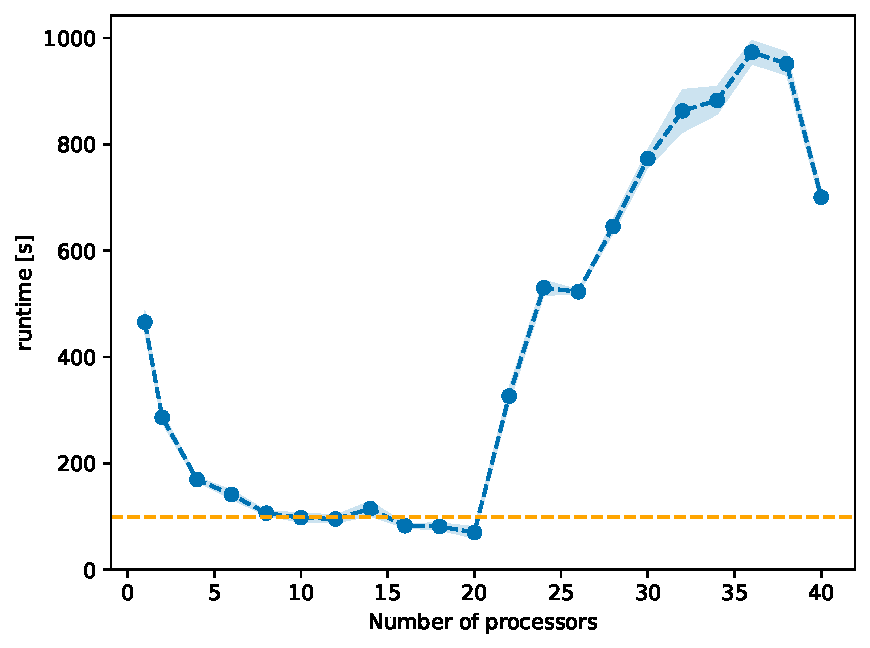
\includegraphics[width=\textwidth]{plots_scf/si_ompi_bench_nprocs_absolute.pdf}
\end{subfigure}
\begin{subfigure}[b]{0.32\textwidth}
    \centering
    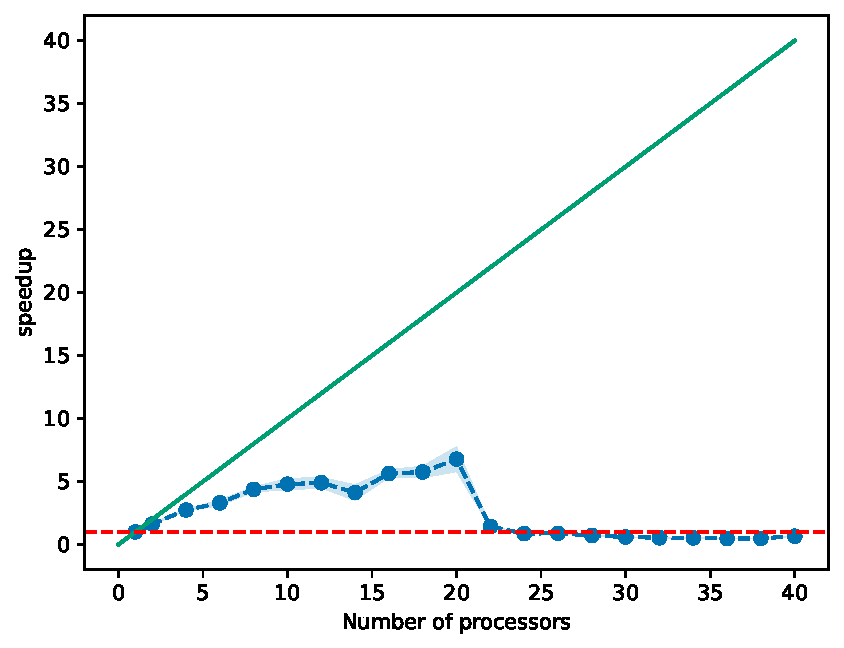
\includegraphics[width=\textwidth]{plots_scf/si_ompi_bench_nprocs_speedup.pdf}
\end{subfigure}
\begin{subfigure}[b]{0.32\textwidth}
    \centering
    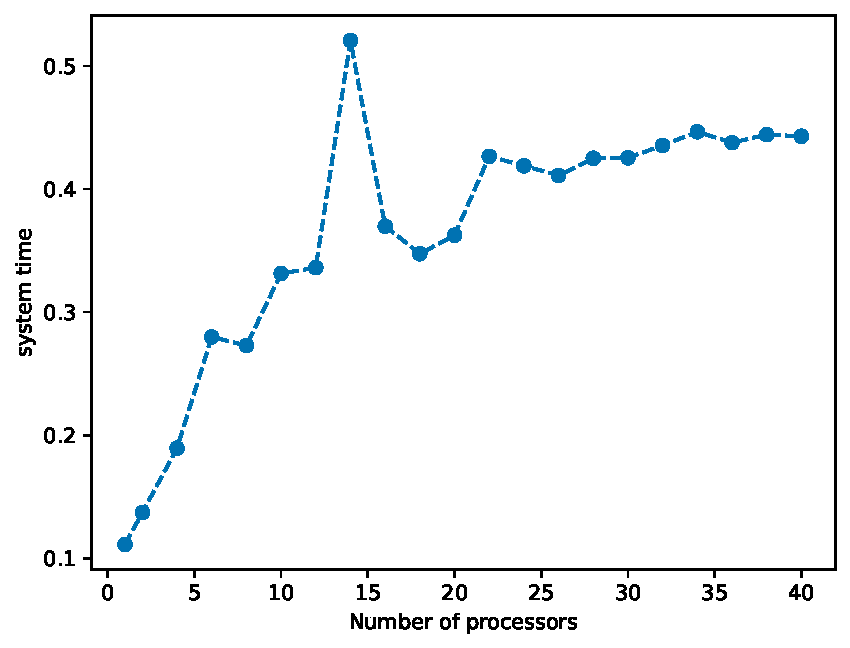
\includegraphics[width=\textwidth]{plots_scf/si_ompi_bench_nprocs_wait.pdf}
\end{subfigure}
\caption{Baseline scaling test on the Si benchmarking system \emph{\QE 7.0, \gls{openmpi} 4.1.0, \texttt{nk 1} and \texttt{nd 1}}}
\label{fig:scaling_ompi_nprocs_si}
\end{figure}

\begin{figure}[h!]
\begin{subfigure}[b]{0.32\textwidth}
    \centering
    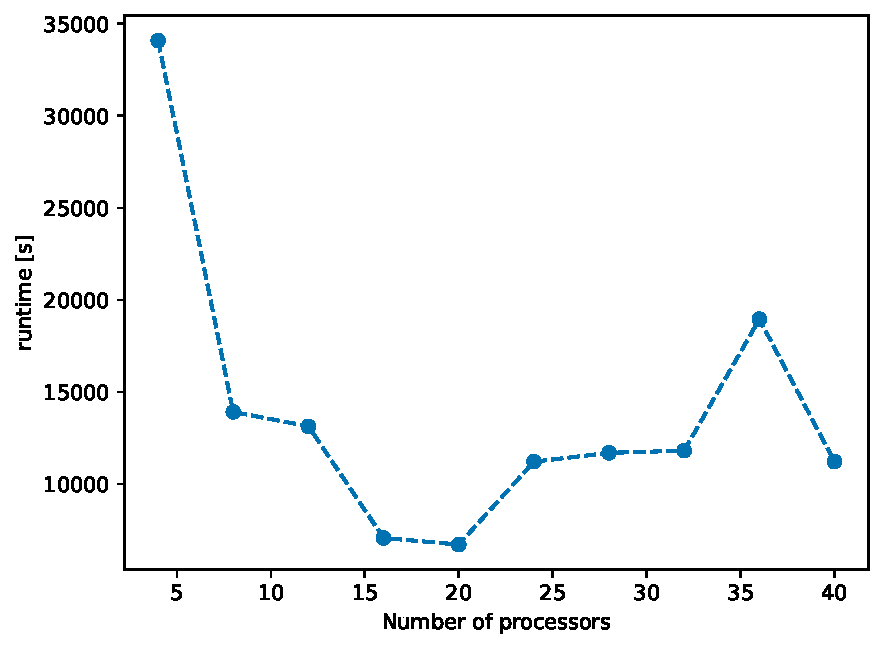
\includegraphics[width=\textwidth]{plots_scf/TaS2_ompi_bench_nprocs_absolute.pdf}
\end{subfigure}
\begin{subfigure}[b]{0.32\textwidth}
    \centering
    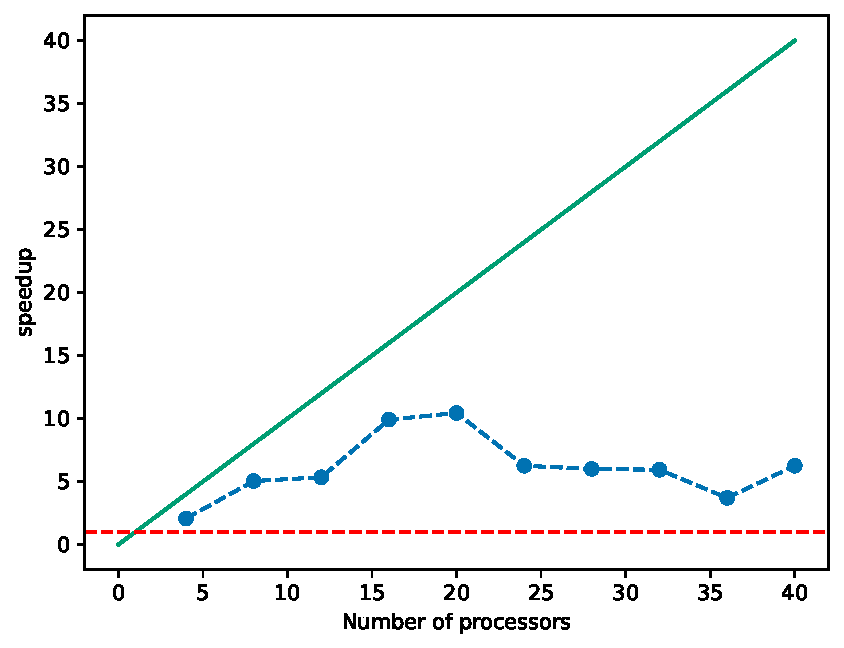
\includegraphics[width=\textwidth]{plots_scf/TaS2_ompi_bench_nprocs_speedup.pdf}
\end{subfigure}
\begin{subfigure}[b]{0.32\textwidth}
    \centering
    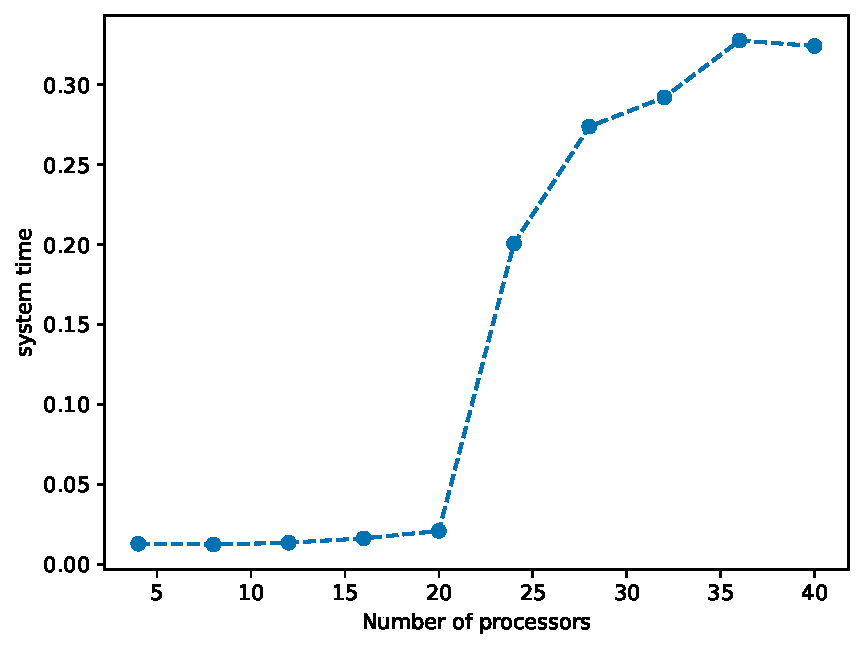
\includegraphics[width=\textwidth]{plots_scf/TaS2_ompi_bench_nprocs_wait.pdf}
\end{subfigure}
\caption{Baseline scaling test on the TaS2 benchmarking system \emph{\QE 7.0, OpenMPI 4.1.0, \texttt{nk 1} and \texttt{nd 1}}}
\label{fig:scaling_ompi_nprocs_tas2}
\end{figure}

\todo{graphics dont look good like that: different heights and too small when 3 side to side}

Three different metrics of scalability are pictured in \ref{fig:scaling_ompi_nprocs}.
\begin{itemize}
    \item runtime: absolute runtime (walltime) of the compute job
    \item speedup: runtime divided by runtime of the job on a single core
    \item system time: percentage of wall time used by system tasks, e.g. writing to disk, etc. (calculated as (walltime - cputime) / walltime)
\end{itemize}
For further analysis mainly speedup will be used as a metric of scalability, because it lends itself to easy interpretation: optimal scalability is achieved when the speedup scales linearly with the number of processors (with a slope of one), as discussed in ch. \ref{sec:parallel_computing}.
This on the one hand necessarily implies good parallelization and a lower runtime for more processors used, but the other two parameters should also always be considered.

As an example, for a problem with a single core runtime of \(\SI{600}{\s}\), a speedup of 100 would mean a runtime of \(\SI{6}{\s}\), whereas a speedup of 200 would mean a runtime of \(\SI{3}{\s}\).
Even with optimal scaling, the 100 processors needed for the speedup of 200 could be considered wasted for just \(\SI{3}{s}\) of saved time.
On the other hand, for a problem with a single core runtime of \(\SI{2400}{\hour}\), the difference between a speedup of 100 (runtime \(\SI{24}{\hour}\)) and 200 (runtime \(\SI{12}{\hour}\)) is the difference between needing to wait a whole day for the calculation and being able to let the job run overnight and continue working in the morning, so using 100 more processors for that can be considered a good use of resources.

On a single node, both the Si and TaS2 calculations show good, but not perfect scaling behavior: the speedup does approximately scale linearly with the number of processors, but the slope is closer to \(\frac{1}{2}\), than 1.
Even though the scaling behavior is not perfect, there is just a small, almost constant amount of runtime used by system calls, this speaks for good parallelization.
As discussed in sec. \ref{sec:parallel_computing}, startup time is an unavoidable part of every parallel program, so a constant amount of time used not for calculations is expected, bad parallelization on the other hand shows itself by introducing waiting times between processors, which makes the waiting time in some way dependent on the number of processors.

When using more than one node, not only does the scaling get worse, the execution needs longer than on a single core for the Si system, with a marginally better performance for the TaS2 system.
This is also seen in the plots of system time. The percentage of time used for tasks not directly related to calculations goes from a near constant value for under 20 processors to 50\% of the execution time for the Si system and 35\% for the TaS2 system.

These scaling tests pose now two questions to be answered:
\begin{itemize}
    \item Is better scaling on a single node possible?
    \item How can acceptable scaling over more than one node be achieved?
\end{itemize}

\section{Testing different compilers and mathematical libraries}

A first strategy for solving issues with parallelization is trying different compilers and mathematical libraries.
In the PHYSnet cluster a variety of software packages is available.
As discussed in sec. \ref{sec:qe}, for the compilation of \QE 

For testing \QE will be compiled using the following software combinations:
\begin{itemize}
    \item \gls{openmpi} 4.1.0 and \gls{openblas}
    \item \gls{openmpi} 4.1.0 and \gls{scalapack}
    \item \gls{oneapi} 2021.4 (includes Intel MPI, Fortran and C compilers as well as Intel MKL, a scalable mathematical library)
\end{itemize}

\begin{figure}[h!]
\begin{subfigure}[b]{0.4\textwidth}
    \centering
    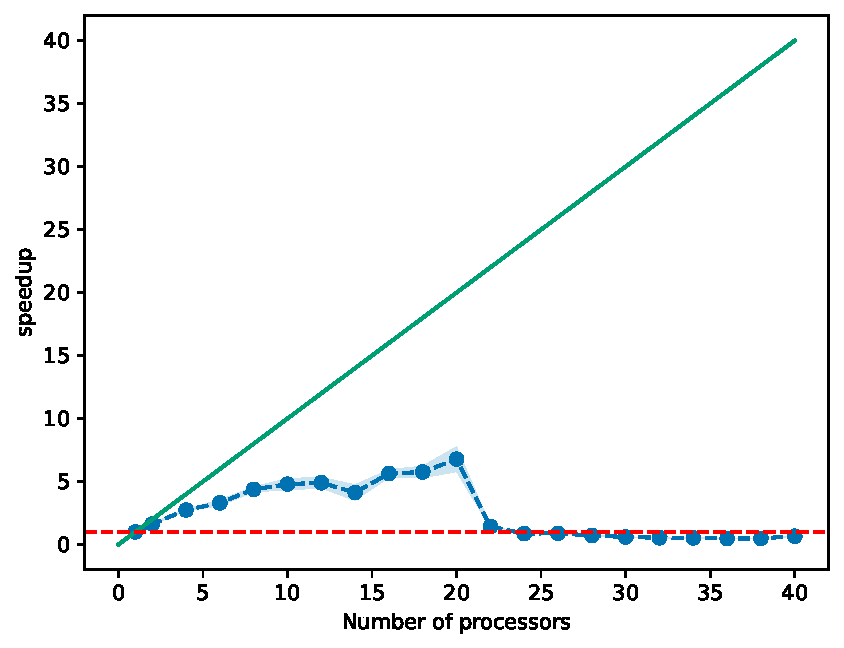
\includegraphics[width=\textwidth]{plots_scf/si_ompi_bench_nprocs_speedup.pdf}
    \subcaption{\gls{openmpi}}
\end{subfigure}
\begin{subfigure}[b]{0.4\textwidth}
    \centering
    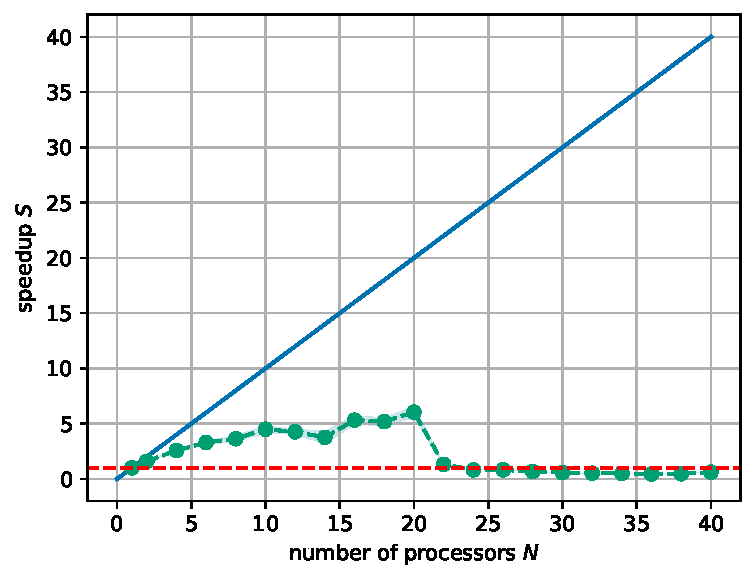
\includegraphics[width=\textwidth]{plots_scf/si_openblas_bench_nprocs_speedup.pdf}
    \subcaption{\gls{openmpi} + \gls{openblas}}
\end{subfigure}
\begin{subfigure}[b]{0.4\textwidth}
    \centering
    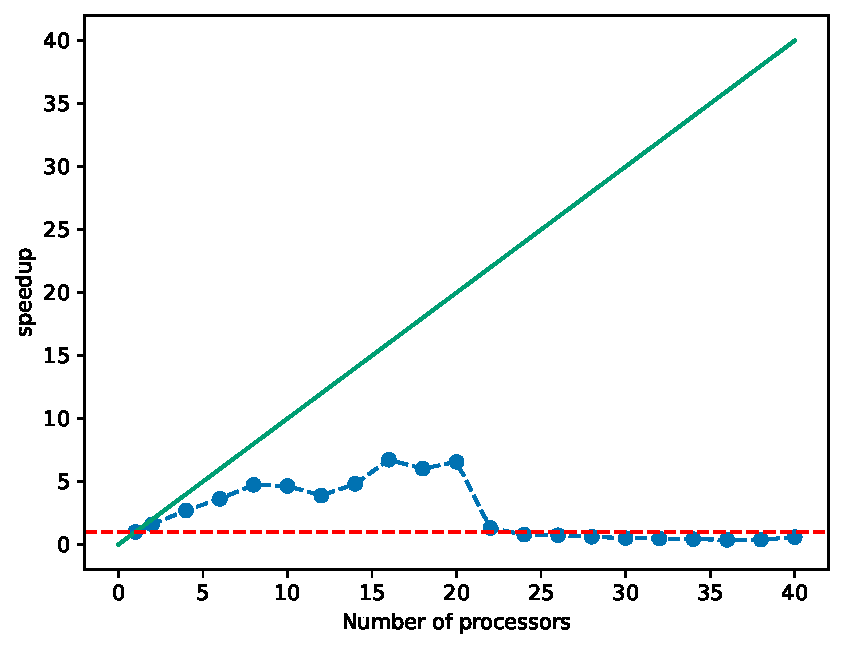
\includegraphics[width=\textwidth]{plots_scf/si_scalapack_bench_nprocs_speedup.pdf}
    \subcaption{\gls{openmpi} + \gls{scalapack}}
\end{subfigure}
\begin{subfigure}[b]{0.4\textwidth}
    \centering
    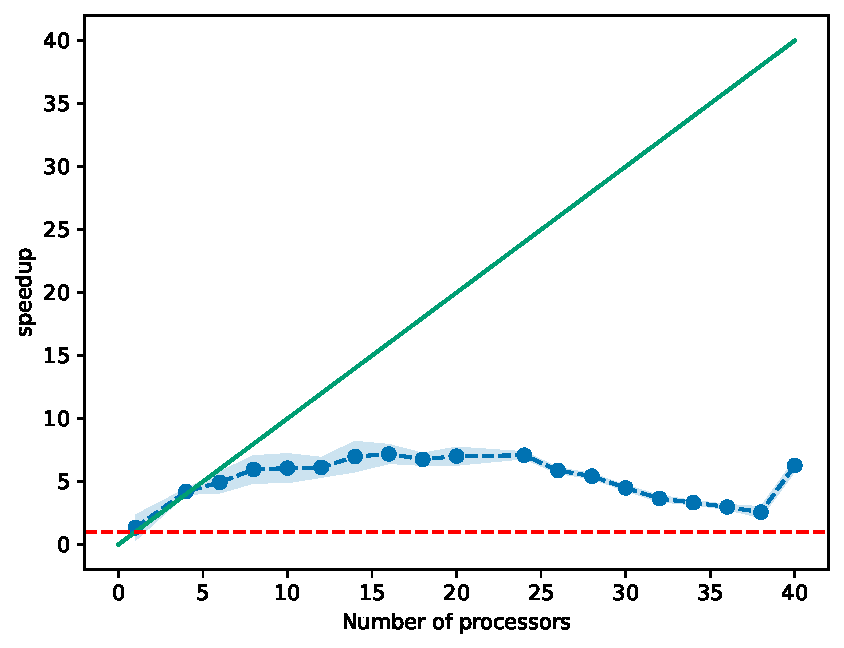
\includegraphics[width=\textwidth]{plots_scf/si_intel_bench_nprocs_speedup.pdf}
    \subcaption{\gls{oneapi}}
\end{subfigure}
\caption{Baseline scaling test with different combinations of compilers and mathematical libraries}
\label{fig:scaling_compilers_nprocs}
\end{figure}

\todo{analysis}

\section{Using the parallelisation parameters of \QE}

As detailed in section \ref{sec:qe}, \QE offers ways to manage how the workload is distributed among the processors.
In \texttt{pw.x} the default plane wave parallelization, k-point-parallelization and linear-algebra parallelization are implemented.

The benchmark pictured in \ref{fig:scaling_nk_si} is set up as follows: for a given number of processors \(N_p\), the parameter \(N_k\) splits the \(N_p\) processors into \(N_k\) processors pools.
As the number of processors in one pool has to be a whole number, only certain combinations of \(N_p\) and \(N_k\) are possible, for example \(N_p = 32\) could be split into processor pools of size 2 with \(N_k = 16\), size 8 with \(N_k = 4\) or size 16 with \(N_k = 2\).
This leads to choosing the size of the processor pools as a variable, not the parameter \texttt{nk}.
Fig. \ref{fig:scaling_nk_si} shows the scaling for poolsizes 2, 8 and 16 for \QE being compiled with OpenMPI/Scalapack and Intel oneAPI.
This choice of pool sizes showcases the smallest pool size possibly (namely 2), as well as a bigger pool size with 16, that still gives rise to a few data points over the chosen range of processors.

\begin{figure}[h!]
\begin{subfigure}[b]{0.49\textwidth}
    \centering
    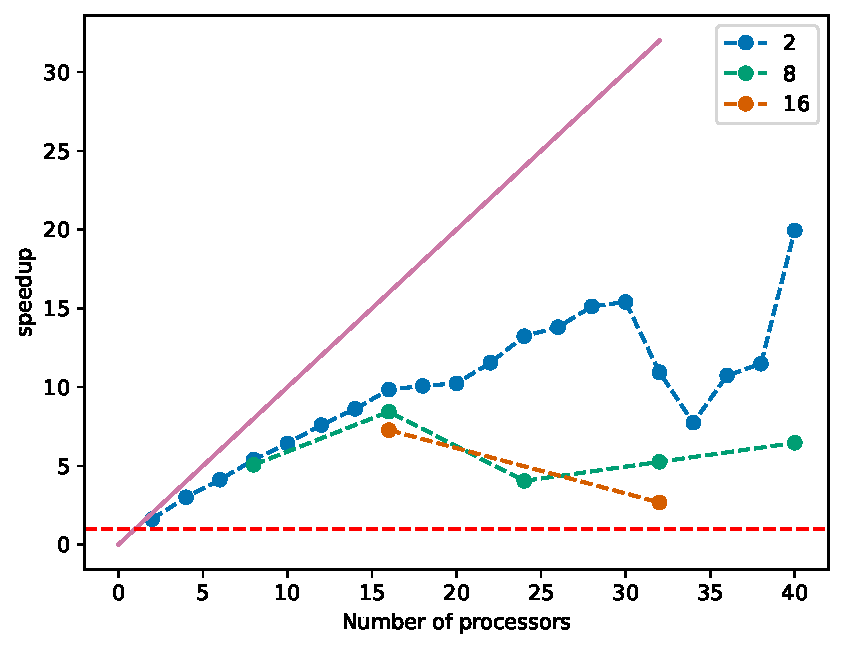
\includegraphics[width=\textwidth]{plots_scf/si_ompi_bench_nk_speedup.pdf}
    \subcaption{\gls{openmpi} + \gls{scalapack}}
\end{subfigure}
\begin{subfigure}[b]{0.49\textwidth}
    \centering
    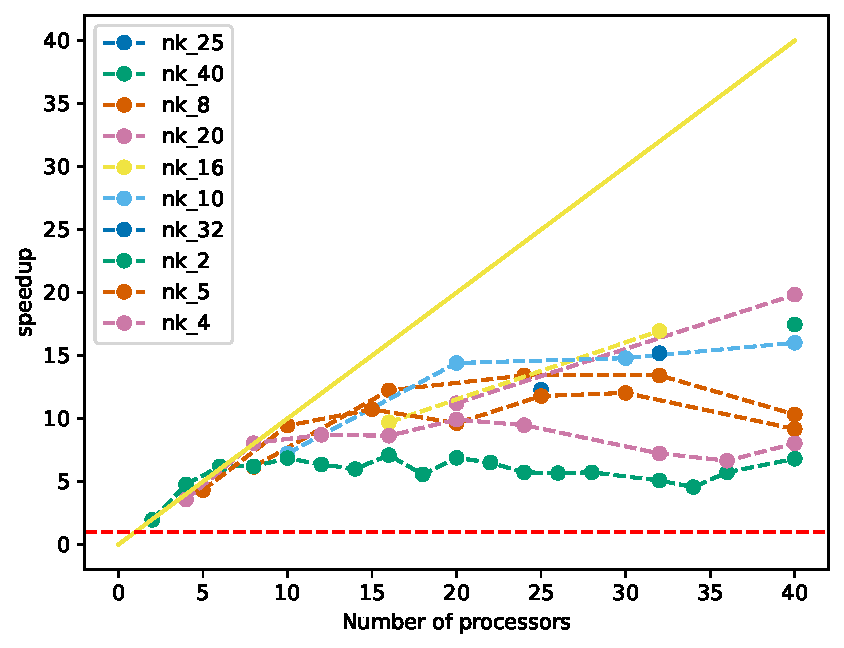
\includegraphics[width=\textwidth]{plots_scf/si_intel_bench_nk_speedup.pdf}
    \subcaption{\gls{oneapi}}
\end{subfigure}
\caption{Benchmark with k-point parallelization for the Si benchmarking system with 3 different sizes of processor pools}
\label{fig:scaling_nk_si}
\end{figure}

Fig. \ref{fig:scaling_nk_si} shows that using k parallelization with a pool size of 2 significantly improves the scaling behavior, not only on one node, but especially over more than one node.

\todo{analysis}

Another important conclusion to draw out of fig. \ref{fig:scaling_nk_si} is the impact of using Intels compiler instead of OpenMPI, as that factor alone speeds up the calculation by a factor of 2 over the whole range of processors.

The same scaling test is applied to the TaS2 system in fig. \ref{fig:scaling_nk_tas2}, with the same list of pool sizes, but over a wider range of processors.

\begin{figure}[h!]
    \centering
    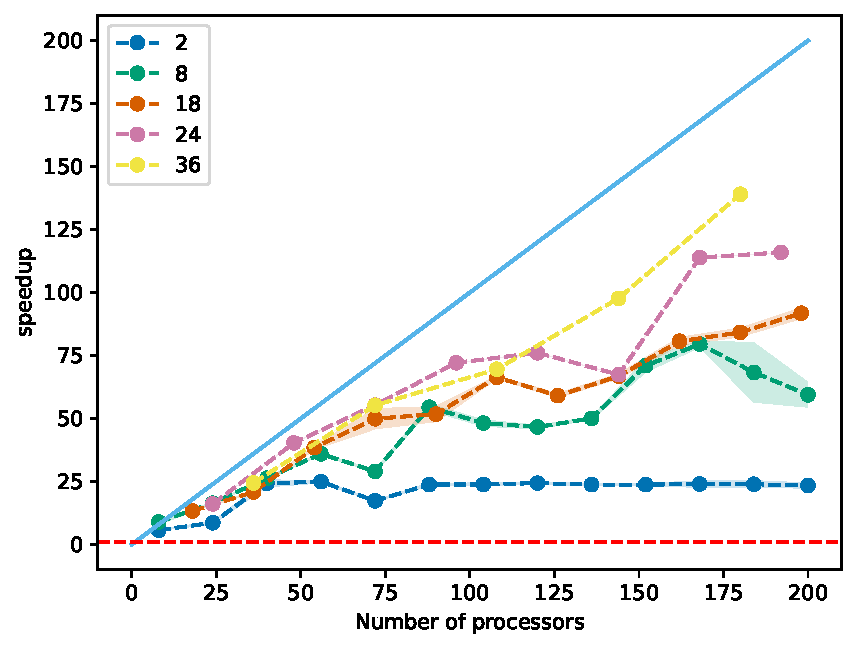
\includegraphics[width=0.8\textwidth]{plots_scf/TaS2_intel_bench_nk_speedup.pdf}
    \caption{Benchmark with k-point parallelization for the TaS2 benchmarking system}
    \label{fig:scaling_nk_tas2}
\end{figure}

Remarkably, the scaling behavior is swapped in comparison to \ref{fig:scaling_nk_si}, as the pool size 2 saturates fast and the bigger pool sizes show way better scaling behavior.
Furthermore, there are instances of better than linear scaling, which according to \QE docs can be attributed to better caching of data.

It can also be instructive to look at the idle time for this benchmark to judge the quality of parallelization. 

\begin{figure}[h!]
    \centering
    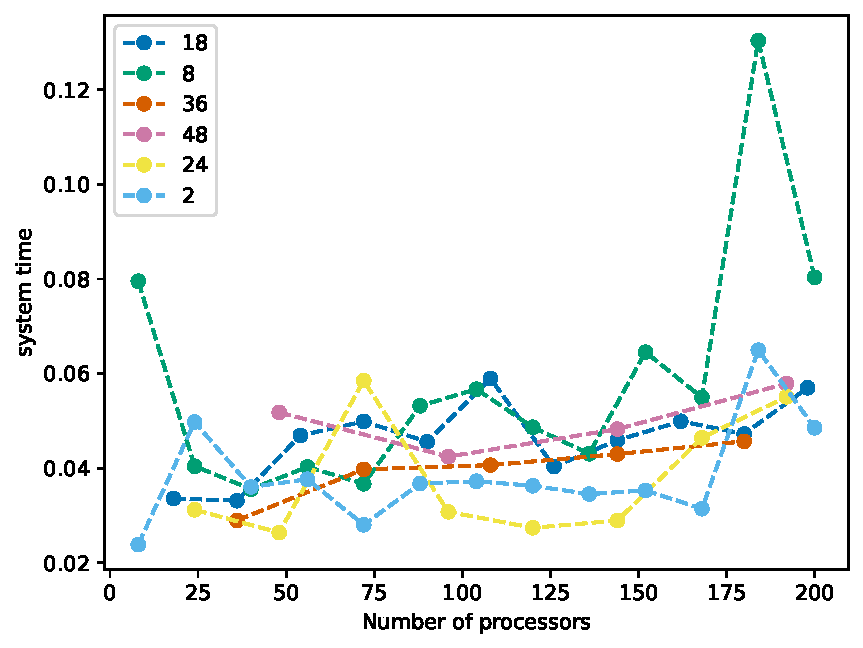
\includegraphics[width=0.8\textwidth]{plots_scf/TaS2_intel_bench_nk_wait.pdf}
    \caption{Idle time for the k point parallelization benchmark for the TaS2 system}
    \label{fig:scaling_nk_tas2_wait}
\end{figure}

Fig. \ref{fig:scaling_nk_tas2_wait} shows a distribution of idle times between \(\SI{1}{\percent}\) and \(\SI{4}{\percent}\) of the whole wall time, without any kind of systemic increase over any range of processors.
This means the parallelization is as good as possible for these 

\subsection{Comparison with calculations on the HLRN cluster}

\subsection{Conclusion: Parameters for optimal scaling}

\end{document}